\documentclass[11pt]{article}
\usepackage[textwidth=18.0cm, textheight=23.0cm, top=2.0cm]{geometry}
\usepackage{pst-all}
\usepackage{amssymb}
\usepackage{tikz}
\usepackage{underscore}\begin{document}
\pagestyle{empty}


ClassName: \underline{\textbf{Class_07.2bp-17}}
\par
BinSize: \underline{\textbf{100 × 100}}
\par
ReduceSize: \underline{\textbf{100 × 100}}
\par
TypeNum: \underline{\textbf{40}}
\par
Num: \underline{\textbf{40}}
\par
OutS: \underline{\textbf{110000}}
\par
InS: \underline{\textbf{95525}}
\par
Rate: \underline{\textbf{0.868}}
\par
UB: \underline{\textbf{11}}
\par
LB0: \underline{\textbf{11}}
\par
LB: \underline{\textbf{11}}
\par
LBWithCut: \underline{\textbf{11}}
\par
NodeCut: \underline{\textbf{0}}
\par
ExtendedNodeCnt: \underline{\textbf{1}}
\par
GenNodeCnt: \underline{\textbf{1}}
\par
PrimalNode: \underline{\textbf{0}}
\par
ColumnCount: \underline{\textbf{11}}
\par
TotalCutCount: \underline{\textbf{0}}
\par
RootCutCount: \underline{\textbf{0}}
\par
LPSolverCnt: \underline{\textbf{1}}
\par
PricingSolverCnt: \underline{\textbf{0}}
\par
BranchAndBoundNum: \underline{\textbf{1}}
\par
isOpt: \underline{\textbf{true}}
\par
TimeOnPrimal: \underline{\textbf{0.000 s}}
\par
TimeOnPricing: \underline{\textbf{0.000 s}}
\par
TimeOnRmp: \underline{\textbf{0.078 s}}
\par
TotalTime: \underline{\textbf{0.125 s}}
\par
\newpage


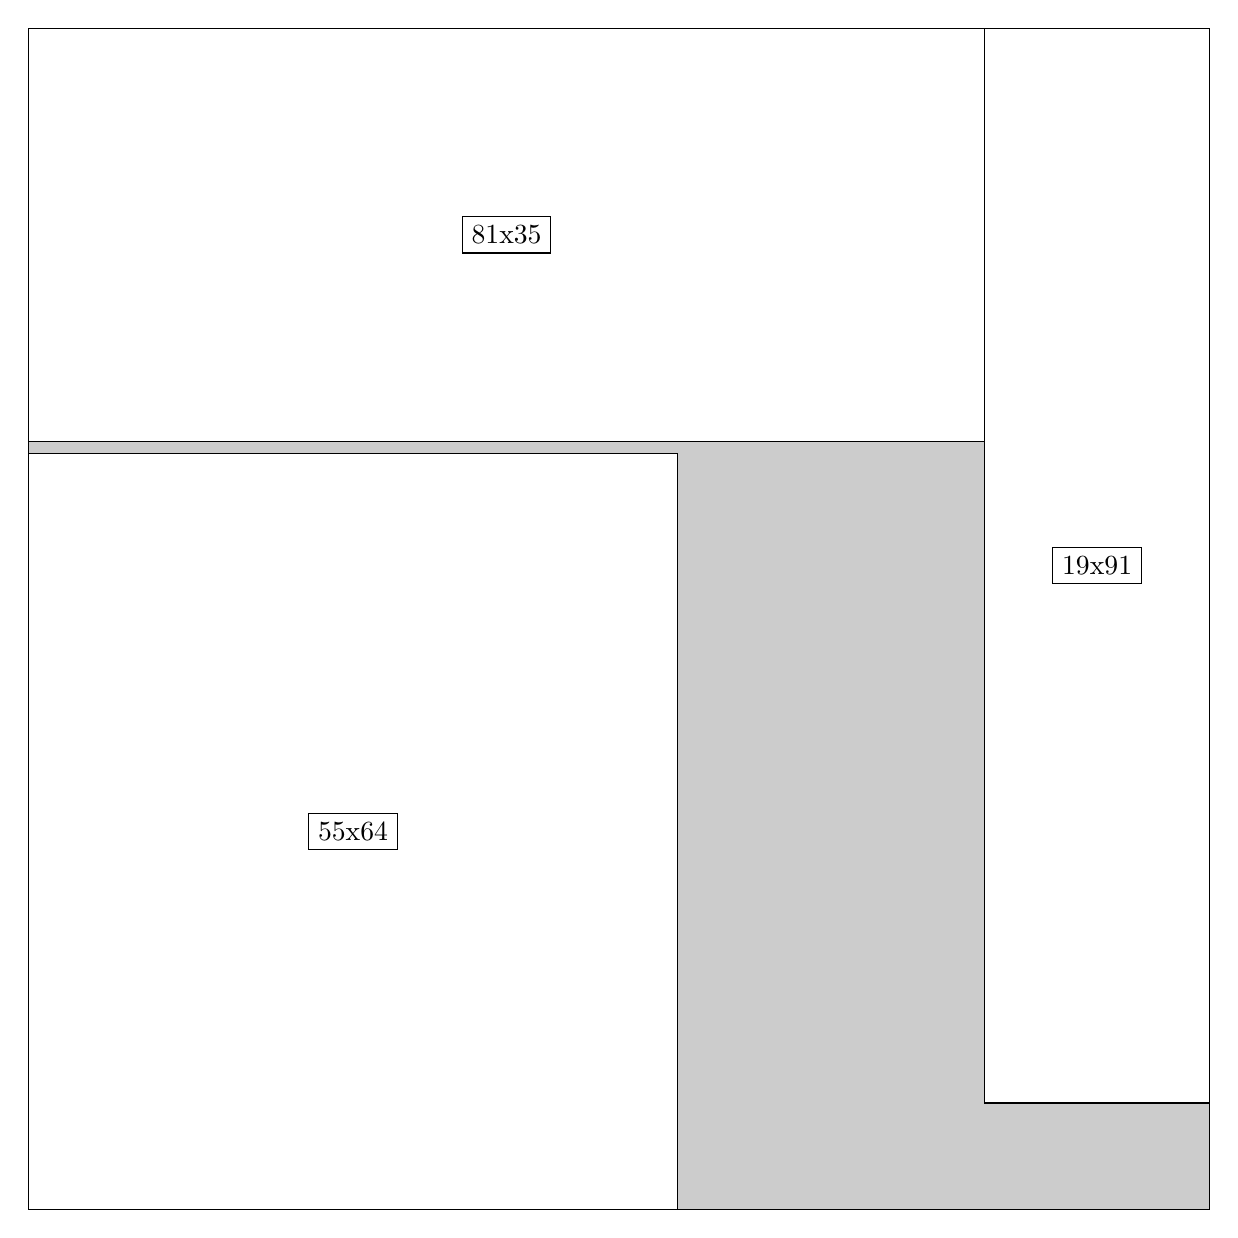
\begin{tikzpicture}[shorten >=1pt,scale=1.0,every node/.style={scale=1.0},->]
\tikzstyle{vertex}=[circle,fill=black!25,minimum size=14pt,inner sep=0pt]
\filldraw[fill=gray!40!white, draw=black] (0,0) rectangle (15.0,15.0);
\foreach \name/\x/\y/\w/\h in {81x35/0.0/9.75/12.15/5.25,19x91/12.15/1.3499999999999999/2.85/13.65,55x64/0.0/0.0/8.25/9.6}
\filldraw[fill=white!40!white, draw=black] (\x,\y) rectangle node[draw] (\name) {\name} ++(\w,\h);
\end{tikzpicture}


w =81 , h =35 , x =0 , y =65 , v =2835
\par
w =19 , h =91 , x =81 , y =9 , v =1729
\par
w =55 , h =64 , x =0 , y =0 , v =3520
\par
\newpage


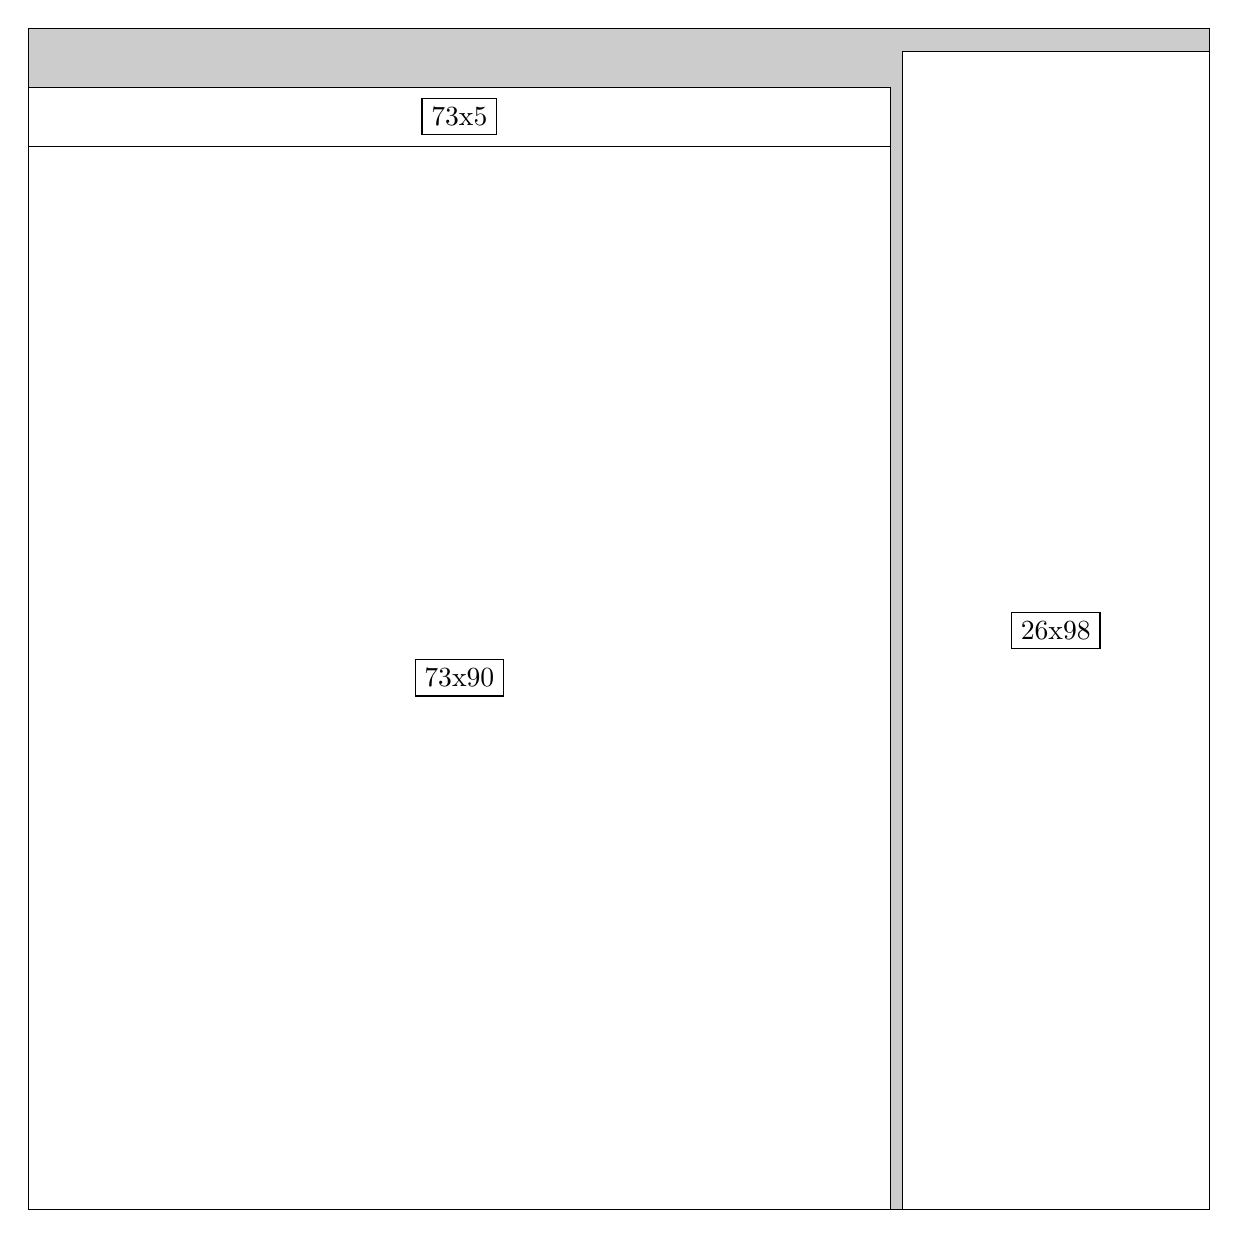
\begin{tikzpicture}[shorten >=1pt,scale=1.0,every node/.style={scale=1.0},->]
\tikzstyle{vertex}=[circle,fill=black!25,minimum size=14pt,inner sep=0pt]
\filldraw[fill=gray!40!white, draw=black] (0,0) rectangle (15.0,15.0);
\foreach \name/\x/\y/\w/\h in {73x90/0.0/0.0/10.95/13.5,26x98/11.1/0.0/3.9/14.7,73x5/0.0/13.5/10.95/0.75}
\filldraw[fill=white!40!white, draw=black] (\x,\y) rectangle node[draw] (\name) {\name} ++(\w,\h);
\end{tikzpicture}


w =73 , h =90 , x =0 , y =0 , v =6570
\par
w =26 , h =98 , x =74 , y =0 , v =2548
\par
w =73 , h =5 , x =0 , y =90 , v =365
\par
\newpage


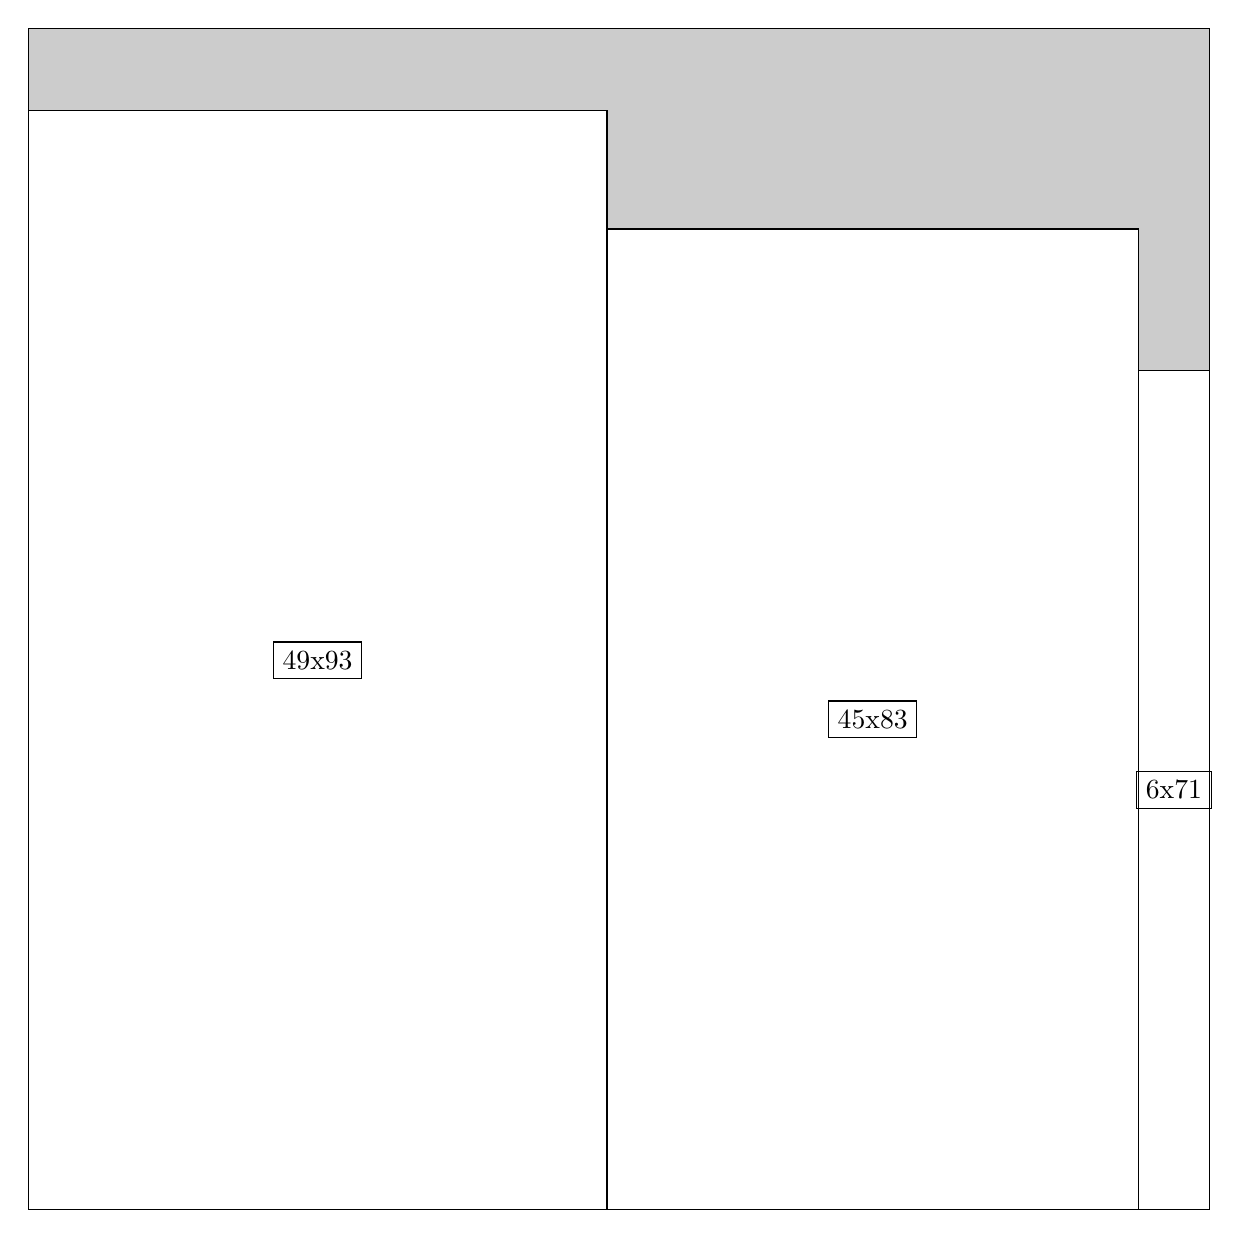
\begin{tikzpicture}[shorten >=1pt,scale=1.0,every node/.style={scale=1.0},->]
\tikzstyle{vertex}=[circle,fill=black!25,minimum size=14pt,inner sep=0pt]
\filldraw[fill=gray!40!white, draw=black] (0,0) rectangle (15.0,15.0);
\foreach \name/\x/\y/\w/\h in {49x93/0.0/0.0/7.35/13.95,45x83/7.35/0.0/6.75/12.45,6x71/14.1/0.0/0.8999999999999999/10.65}
\filldraw[fill=white!40!white, draw=black] (\x,\y) rectangle node[draw] (\name) {\name} ++(\w,\h);
\end{tikzpicture}


w =49 , h =93 , x =0 , y =0 , v =4557
\par
w =45 , h =83 , x =49 , y =0 , v =3735
\par
w =6 , h =71 , x =94 , y =0 , v =426
\par
\newpage


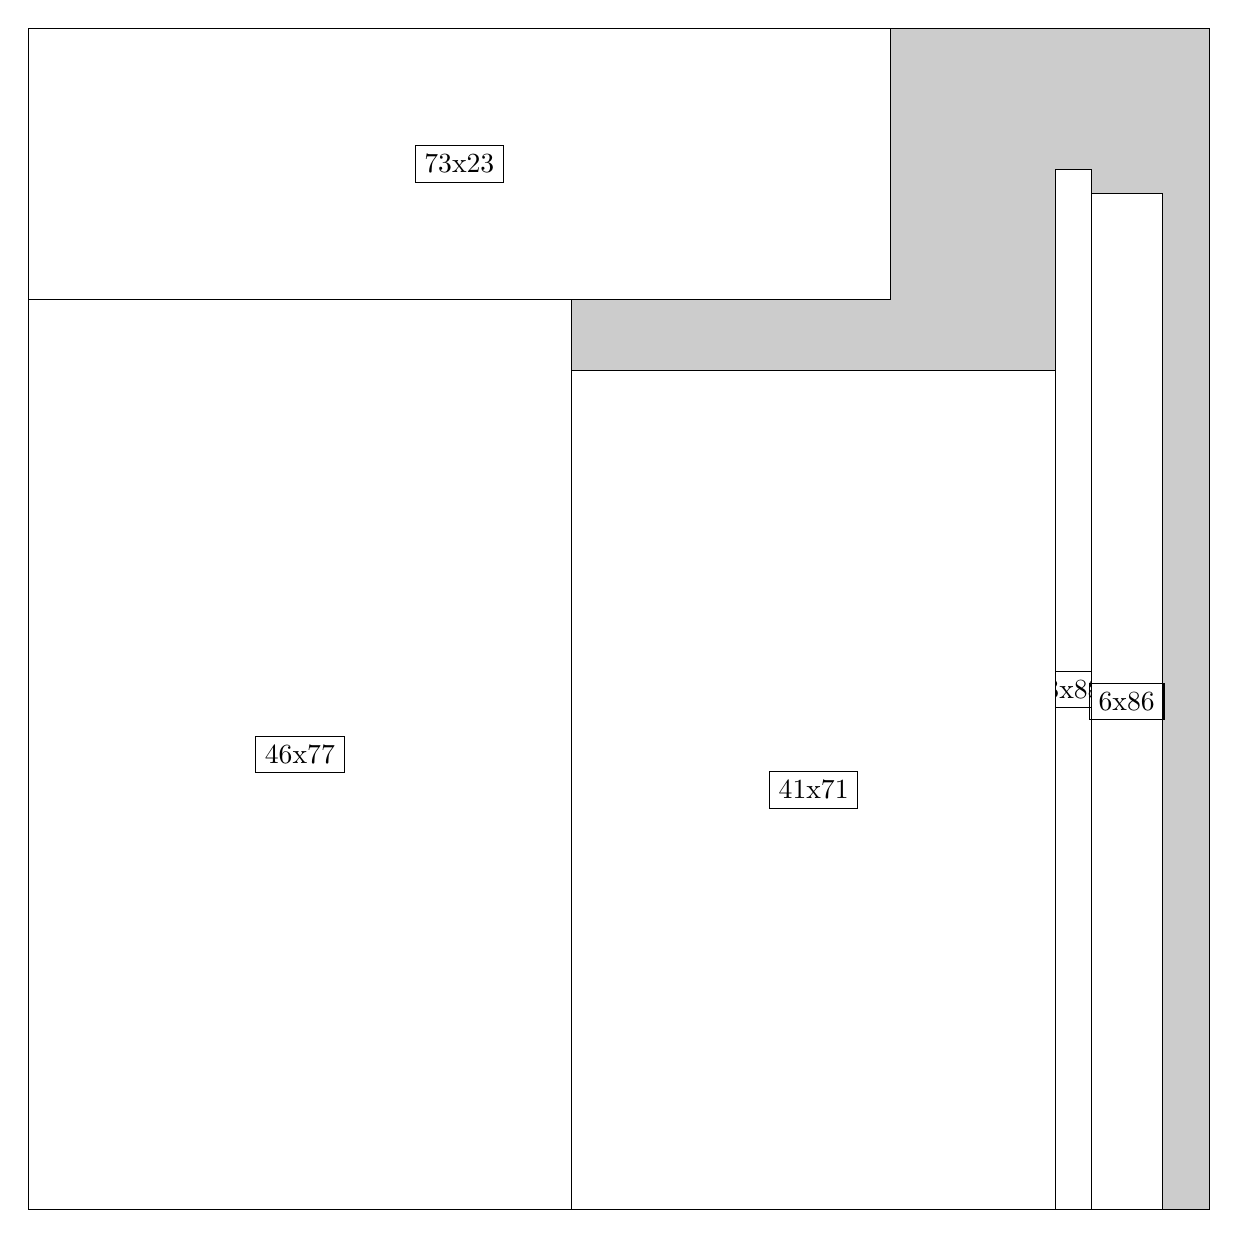
\begin{tikzpicture}[shorten >=1pt,scale=1.0,every node/.style={scale=1.0},->]
\tikzstyle{vertex}=[circle,fill=black!25,minimum size=14pt,inner sep=0pt]
\filldraw[fill=gray!40!white, draw=black] (0,0) rectangle (15.0,15.0);
\foreach \name/\x/\y/\w/\h in {3x88/13.049999999999999/0.0/0.44999999999999996/13.2,46x77/0.0/0.0/6.8999999999999995/11.549999999999999,41x71/6.8999999999999995/0.0/6.1499999999999995/10.65,73x23/0.0/11.549999999999999/10.95/3.4499999999999997,6x86/13.5/0.0/0.8999999999999999/12.9}
\filldraw[fill=white!40!white, draw=black] (\x,\y) rectangle node[draw] (\name) {\name} ++(\w,\h);
\end{tikzpicture}


w =3 , h =88 , x =87 , y =0 , v =264
\par
w =46 , h =77 , x =0 , y =0 , v =3542
\par
w =41 , h =71 , x =46 , y =0 , v =2911
\par
w =73 , h =23 , x =0 , y =77 , v =1679
\par
w =6 , h =86 , x =90 , y =0 , v =516
\par
\newpage


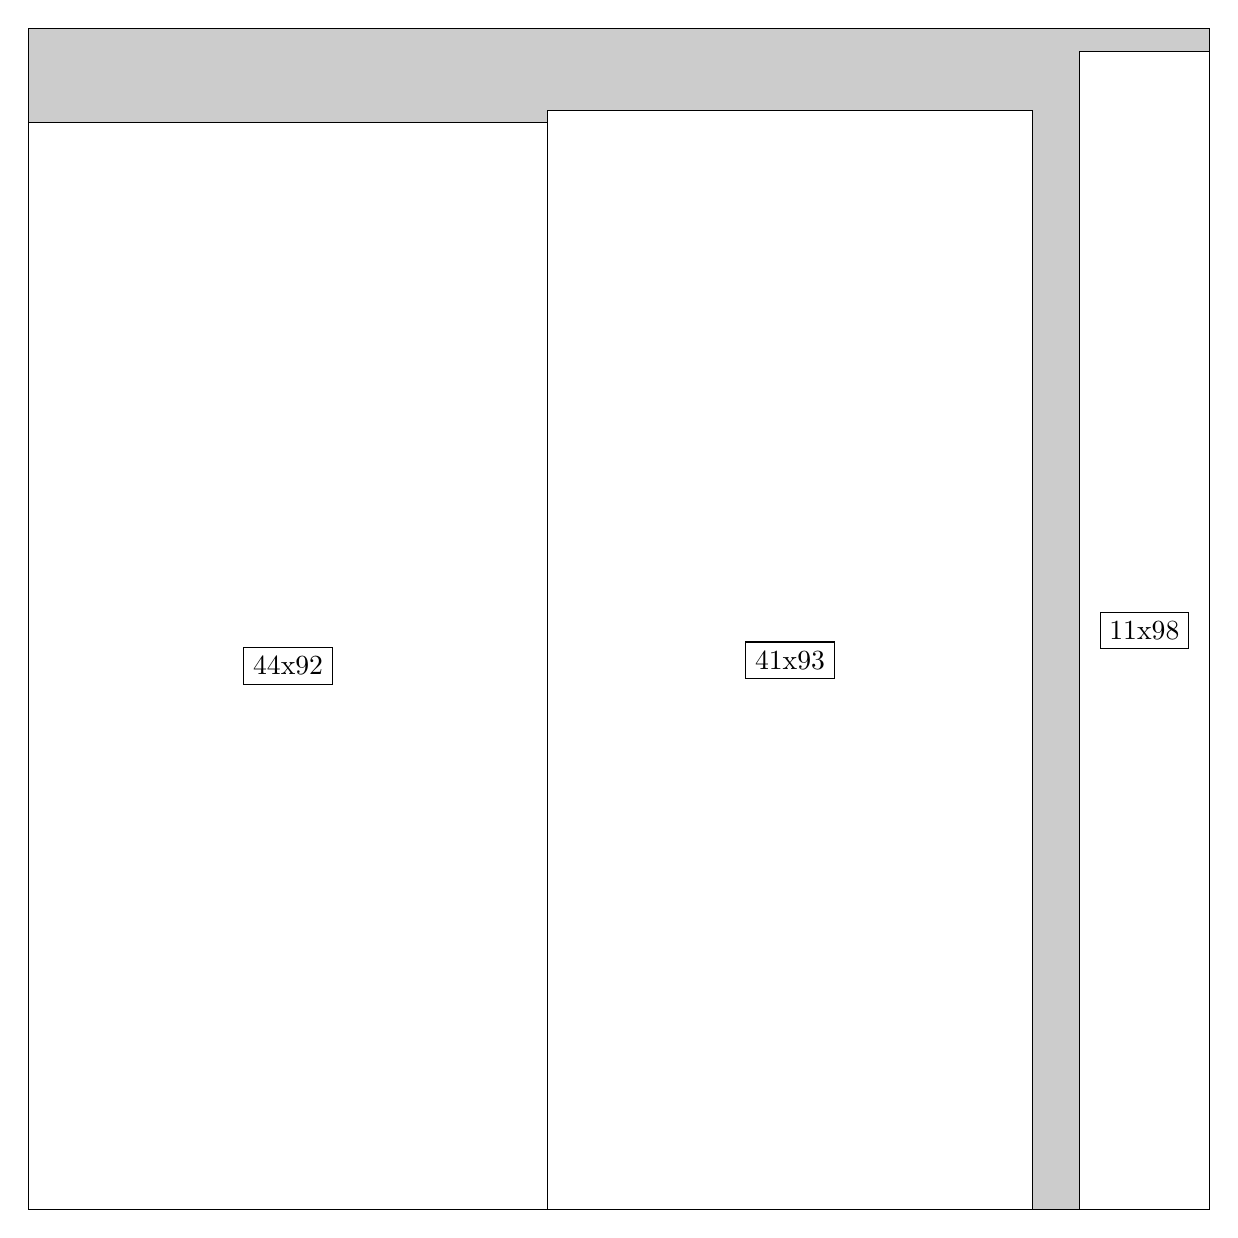
\begin{tikzpicture}[shorten >=1pt,scale=1.0,every node/.style={scale=1.0},->]
\tikzstyle{vertex}=[circle,fill=black!25,minimum size=14pt,inner sep=0pt]
\filldraw[fill=gray!40!white, draw=black] (0,0) rectangle (15.0,15.0);
\foreach \name/\x/\y/\w/\h in {44x92/0.0/0.0/6.6/13.799999999999999,41x93/6.6/0.0/6.1499999999999995/13.95,11x98/13.35/0.0/1.65/14.7}
\filldraw[fill=white!40!white, draw=black] (\x,\y) rectangle node[draw] (\name) {\name} ++(\w,\h);
\end{tikzpicture}


w =44 , h =92 , x =0 , y =0 , v =4048
\par
w =41 , h =93 , x =44 , y =0 , v =3813
\par
w =11 , h =98 , x =89 , y =0 , v =1078
\par
\newpage


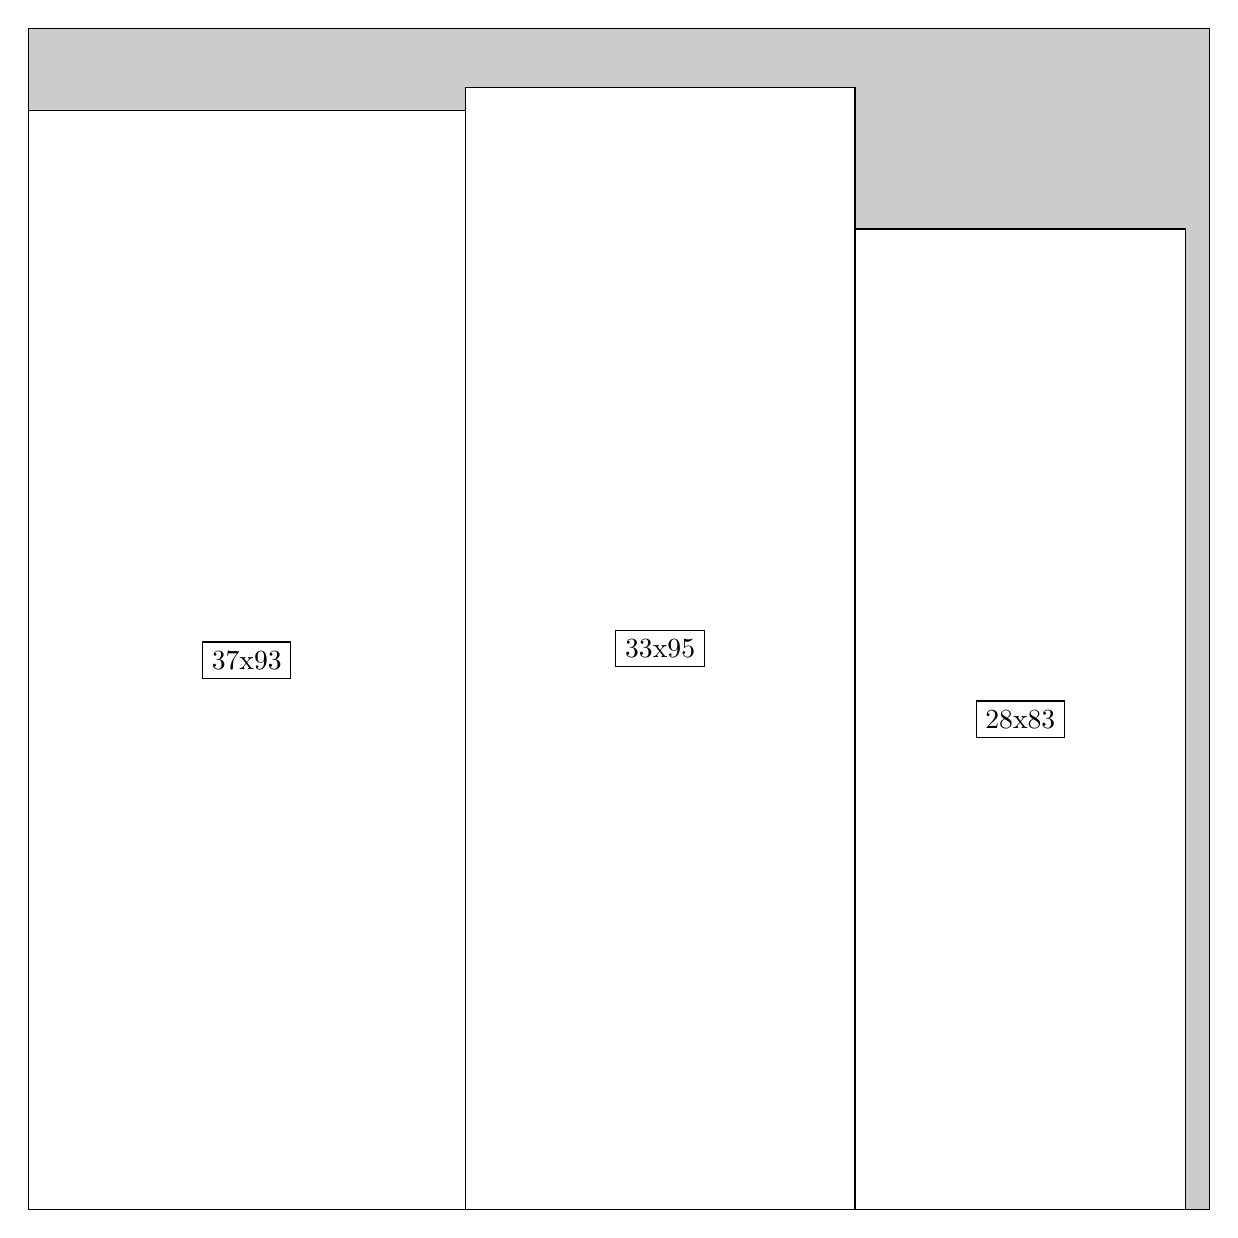
\begin{tikzpicture}[shorten >=1pt,scale=1.0,every node/.style={scale=1.0},->]
\tikzstyle{vertex}=[circle,fill=black!25,minimum size=14pt,inner sep=0pt]
\filldraw[fill=gray!40!white, draw=black] (0,0) rectangle (15.0,15.0);
\foreach \name/\x/\y/\w/\h in {37x93/0.0/0.0/5.55/13.95,33x95/5.55/0.0/4.95/14.25,28x83/10.5/0.0/4.2/12.45}
\filldraw[fill=white!40!white, draw=black] (\x,\y) rectangle node[draw] (\name) {\name} ++(\w,\h);
\end{tikzpicture}


w =37 , h =93 , x =0 , y =0 , v =3441
\par
w =33 , h =95 , x =37 , y =0 , v =3135
\par
w =28 , h =83 , x =70 , y =0 , v =2324
\par
\newpage


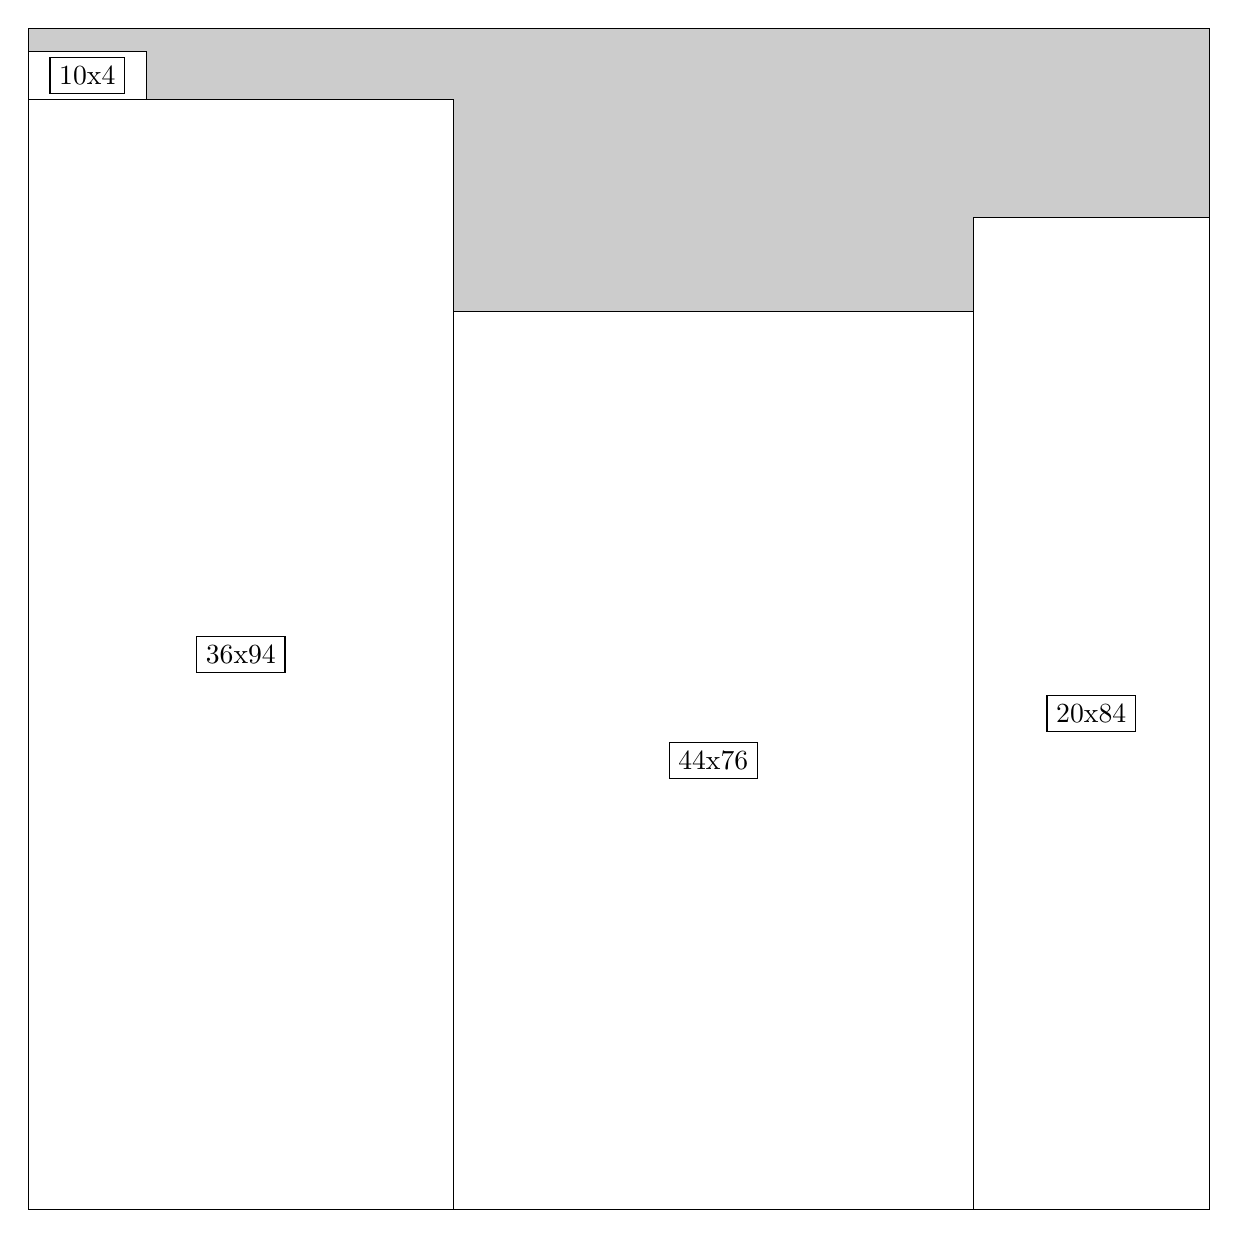
\begin{tikzpicture}[shorten >=1pt,scale=1.0,every node/.style={scale=1.0},->]
\tikzstyle{vertex}=[circle,fill=black!25,minimum size=14pt,inner sep=0pt]
\filldraw[fill=gray!40!white, draw=black] (0,0) rectangle (15.0,15.0);
\foreach \name/\x/\y/\w/\h in {36x94/0.0/0.0/5.3999999999999995/14.1,44x76/5.3999999999999995/0.0/6.6/11.4,20x84/12.0/0.0/3.0/12.6,10x4/0.0/14.1/1.5/0.6}
\filldraw[fill=white!40!white, draw=black] (\x,\y) rectangle node[draw] (\name) {\name} ++(\w,\h);
\end{tikzpicture}


w =36 , h =94 , x =0 , y =0 , v =3384
\par
w =44 , h =76 , x =36 , y =0 , v =3344
\par
w =20 , h =84 , x =80 , y =0 , v =1680
\par
w =10 , h =4 , x =0 , y =94 , v =40
\par
\newpage


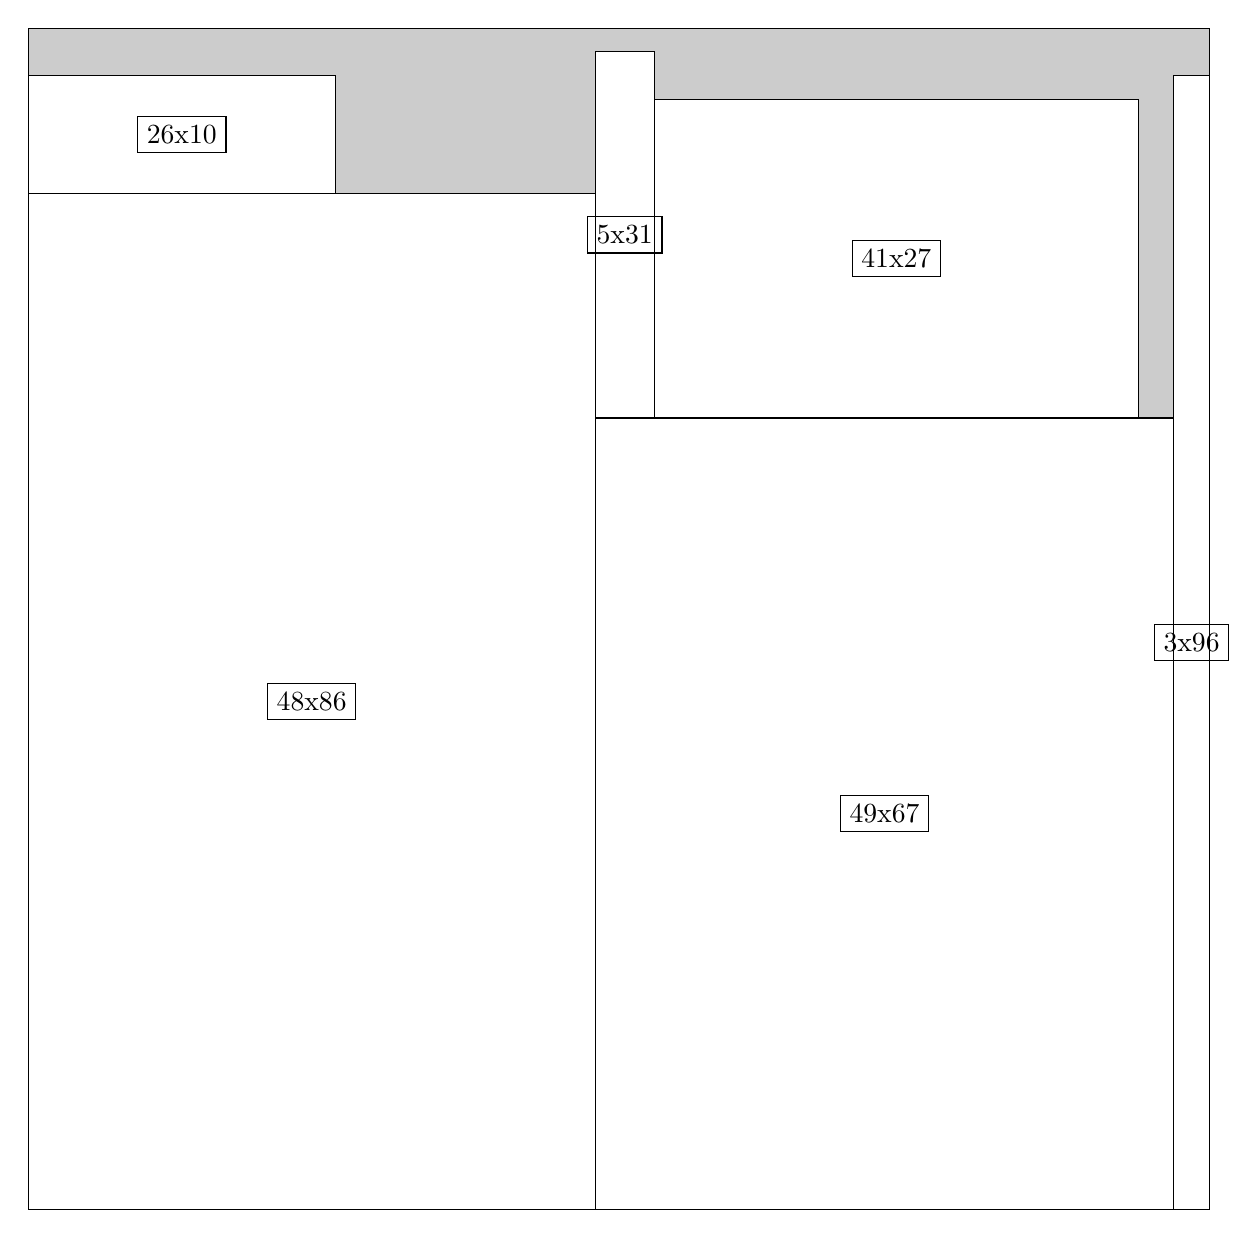
\begin{tikzpicture}[shorten >=1pt,scale=1.0,every node/.style={scale=1.0},->]
\tikzstyle{vertex}=[circle,fill=black!25,minimum size=14pt,inner sep=0pt]
\filldraw[fill=gray!40!white, draw=black] (0,0) rectangle (15.0,15.0);
\foreach \name/\x/\y/\w/\h in {48x86/0.0/0.0/7.199999999999999/12.9,49x67/7.199999999999999/0.0/7.35/10.049999999999999,41x27/7.949999999999999/10.049999999999999/6.1499999999999995/4.05,3x96/14.549999999999999/0.0/0.44999999999999996/14.399999999999999,26x10/0.0/12.9/3.9/1.5,5x31/7.199999999999999/10.049999999999999/0.75/4.6499999999999995}
\filldraw[fill=white!40!white, draw=black] (\x,\y) rectangle node[draw] (\name) {\name} ++(\w,\h);
\end{tikzpicture}


w =48 , h =86 , x =0 , y =0 , v =4128
\par
w =49 , h =67 , x =48 , y =0 , v =3283
\par
w =41 , h =27 , x =53 , y =67 , v =1107
\par
w =3 , h =96 , x =97 , y =0 , v =288
\par
w =26 , h =10 , x =0 , y =86 , v =260
\par
w =5 , h =31 , x =48 , y =67 , v =155
\par
\newpage


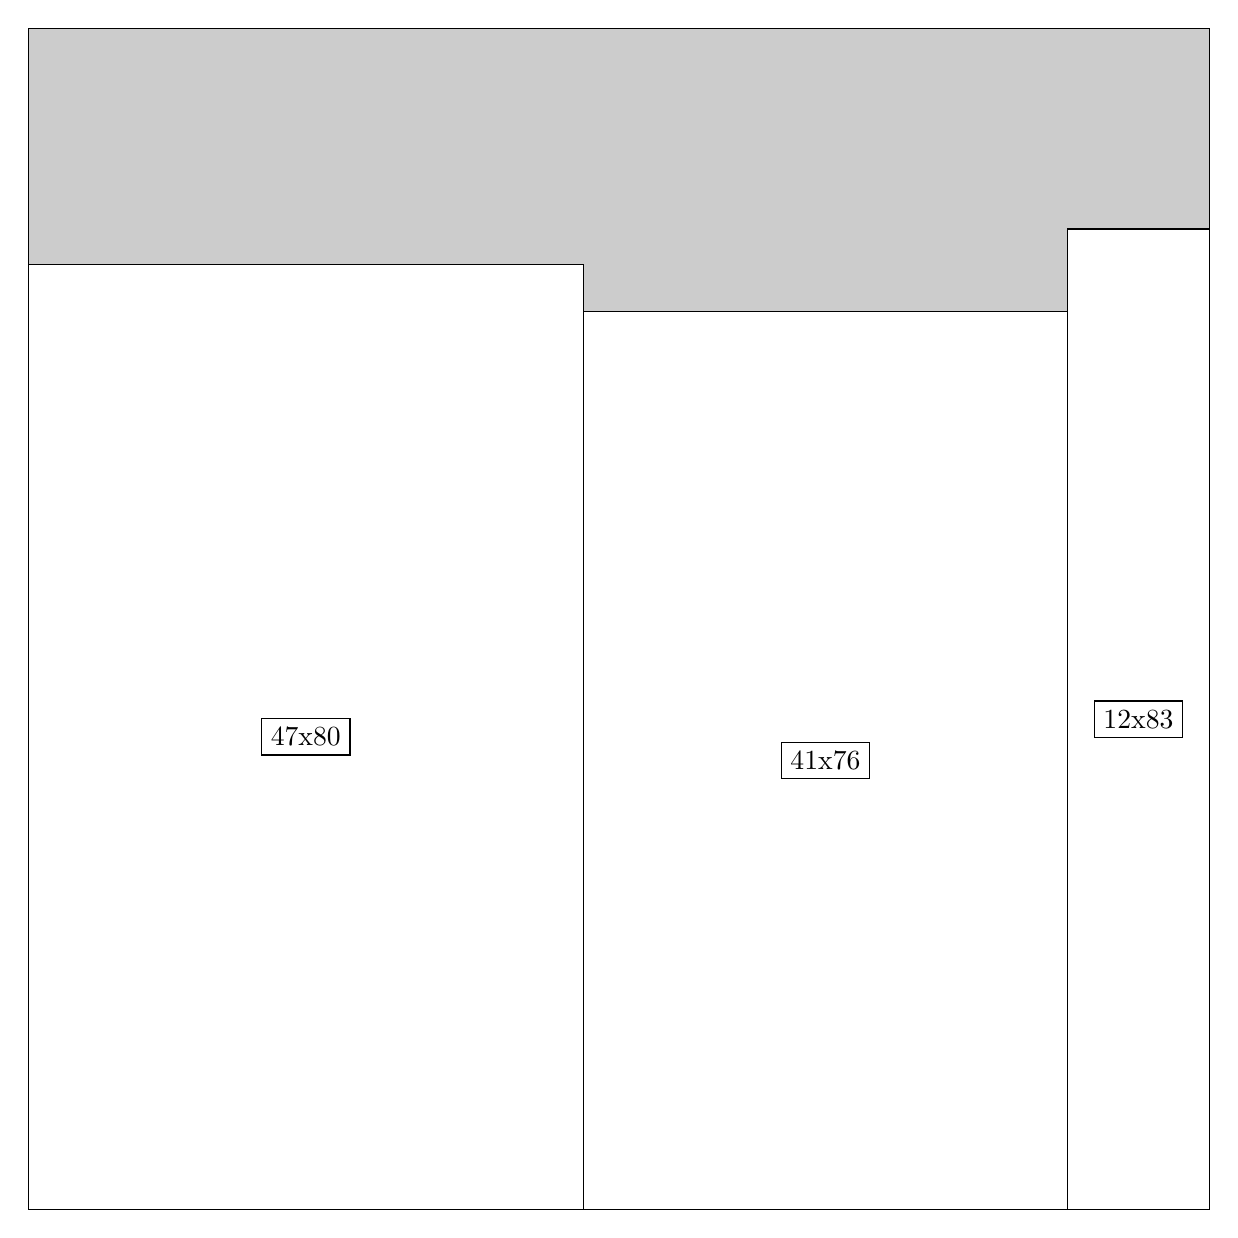
\begin{tikzpicture}[shorten >=1pt,scale=1.0,every node/.style={scale=1.0},->]
\tikzstyle{vertex}=[circle,fill=black!25,minimum size=14pt,inner sep=0pt]
\filldraw[fill=gray!40!white, draw=black] (0,0) rectangle (15.0,15.0);
\foreach \name/\x/\y/\w/\h in {47x80/0.0/0.0/7.05/12.0,41x76/7.05/0.0/6.1499999999999995/11.4,12x83/13.2/0.0/1.7999999999999998/12.45}
\filldraw[fill=white!40!white, draw=black] (\x,\y) rectangle node[draw] (\name) {\name} ++(\w,\h);
\end{tikzpicture}


w =47 , h =80 , x =0 , y =0 , v =3760
\par
w =41 , h =76 , x =47 , y =0 , v =3116
\par
w =12 , h =83 , x =88 , y =0 , v =996
\par
\newpage


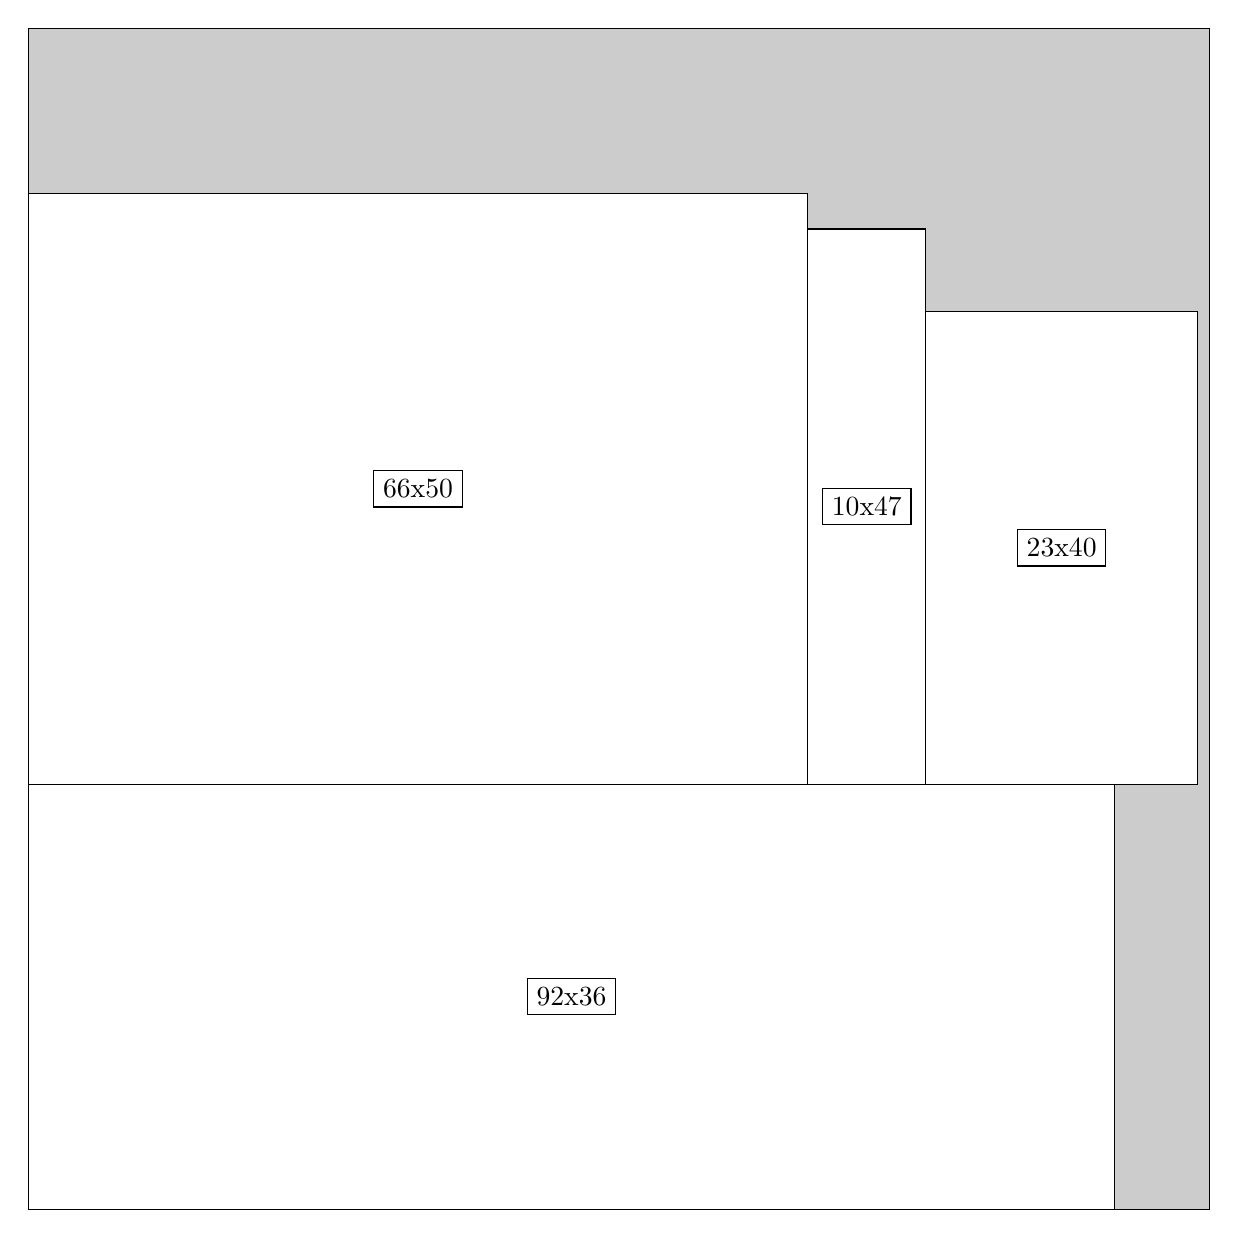
\begin{tikzpicture}[shorten >=1pt,scale=1.0,every node/.style={scale=1.0},->]
\tikzstyle{vertex}=[circle,fill=black!25,minimum size=14pt,inner sep=0pt]
\filldraw[fill=gray!40!white, draw=black] (0,0) rectangle (15.0,15.0);
\foreach \name/\x/\y/\w/\h in {92x36/0.0/0.0/13.799999999999999/5.3999999999999995,66x50/0.0/5.3999999999999995/9.9/7.5,23x40/11.4/5.3999999999999995/3.4499999999999997/6.0,10x47/9.9/5.3999999999999995/1.5/7.05}
\filldraw[fill=white!40!white, draw=black] (\x,\y) rectangle node[draw] (\name) {\name} ++(\w,\h);
\end{tikzpicture}


w =92 , h =36 , x =0 , y =0 , v =3312
\par
w =66 , h =50 , x =0 , y =36 , v =3300
\par
w =23 , h =40 , x =76 , y =36 , v =920
\par
w =10 , h =47 , x =66 , y =36 , v =470
\par
\newpage


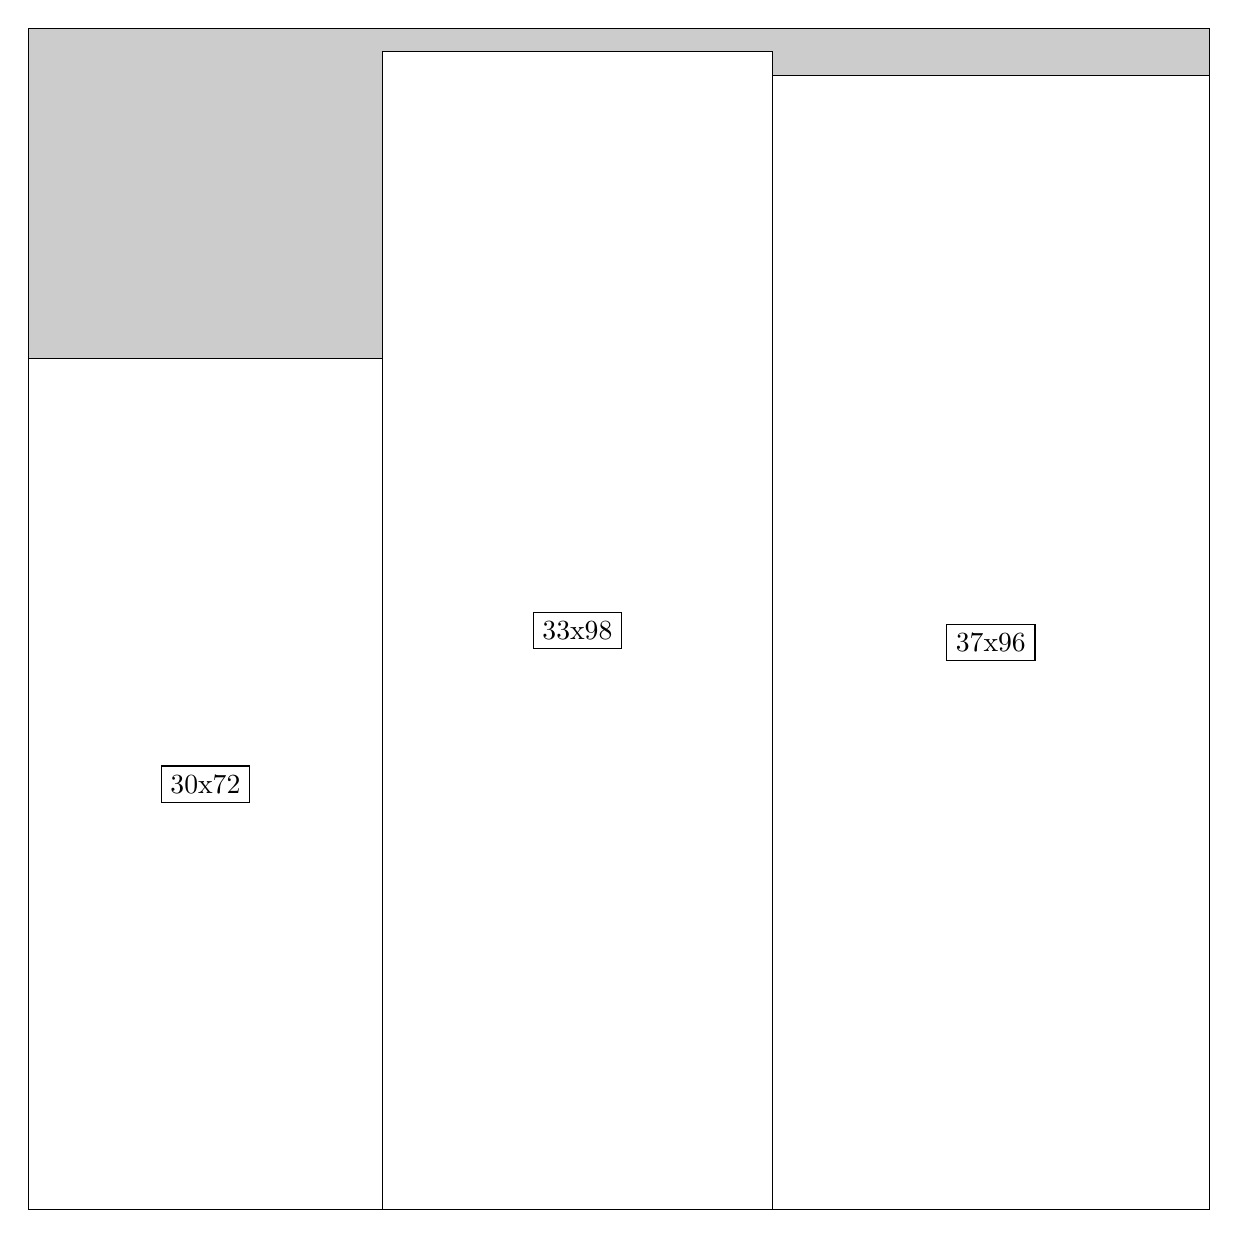
\begin{tikzpicture}[shorten >=1pt,scale=1.0,every node/.style={scale=1.0},->]
\tikzstyle{vertex}=[circle,fill=black!25,minimum size=14pt,inner sep=0pt]
\filldraw[fill=gray!40!white, draw=black] (0,0) rectangle (15.0,15.0);
\foreach \name/\x/\y/\w/\h in {33x98/4.5/0.0/4.95/14.7,30x72/0.0/0.0/4.5/10.799999999999999,37x96/9.45/0.0/5.55/14.399999999999999}
\filldraw[fill=white!40!white, draw=black] (\x,\y) rectangle node[draw] (\name) {\name} ++(\w,\h);
\end{tikzpicture}


w =33 , h =98 , x =30 , y =0 , v =3234
\par
w =30 , h =72 , x =0 , y =0 , v =2160
\par
w =37 , h =96 , x =63 , y =0 , v =3552
\par
\newpage


\end{document}